 \documentclass[t,14pt]{beamer}
 %
 % Packages pour le français
 \usepackage[T1]{fontenc} 
 \usepackage[utf8]{inputenc}
 \usepackage[frenchb]{babel}
 %
 % pour un pdf lisible à l'écran
 % il y a d'autres choix possibles 
 \usepackage{pslatex}
\usetheme{Singapore}
  \usecolortheme{rose}
  \setbeamertemplate{blocks}[rounded][shadow=true]

\title{\textbf{\textit{Extraction et Analyse d'Images}}}
\subtitle{PED}
\author{\scriptsize{Manson Tomy\\
		Mestreau Nicolas\\
		Ridel Fabien\\
		Wen Jun\\
		\vspace{10mm}
		Encadrant : \\
		Laviole Jérémy\\
		}}
\institute{\tiny Université de Bordeaux 1}



\begin{document}

\frame{\titlepage}

%% part 1 - Jun
\section[Présentation]{Présentation}
\AtBeginSection[]{
\begin{frame}{Table of contents}
\small \tableofcontents[currentsection, hideothersubsections]
\end{frame}
}

\begin{frame}{Presentation du projet}
\begin{center}
\vspace{5mm}
Le but de ce projet est la création d'une bibliothèque de vision par l'ordinateur et analyse d'image.

\end{center}
\begin{itemize}
\item Entrée: un flux vidéo de dessin et des images qualitées hautes.
\item Sorti: un image de dessin ou pictogramme .
\end{itemize}
\end{frame}

\begin{frame}{Objectifs}
\begin{center}
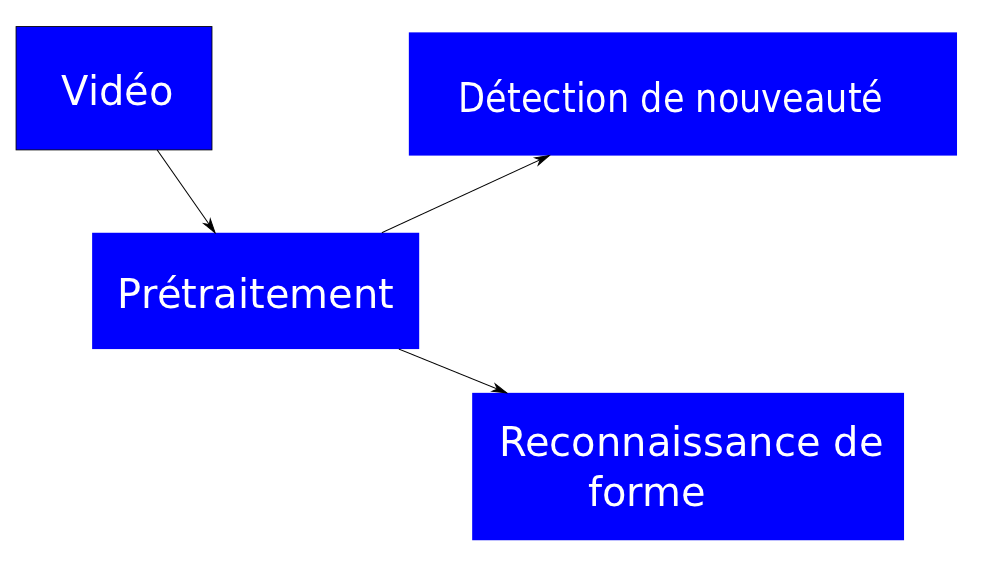
\includegraphics[scale=0.2]{images/dessin.png} 
\\ schéma de processus
\end{center}
\begin{itemize}
\item Augementer la qualité d'image la plus haute possible.
\item Récupérer les nouveautés du dessin.
\item Détecter les formes simples. 
\end{itemize}
\end{frame}


\begin{frame}{Application }
\vspace{2mm}
\begin{itemize}
\item Jeu vidéo Réalité Augementé

\begin{center}
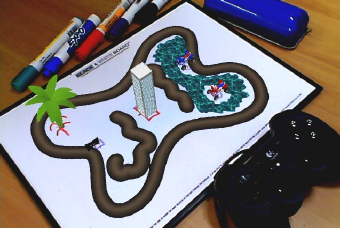
\includegraphics[scale=0.5]{images/sketchchasser.png}
\textit{\\sketchchasser}
\end{center}
\item Auto-scanner 
\end{itemize}
\end{frame}

%% part 2 - Fabien
\section[Pré-traitement]{Pré-traitement}
\vspace{5mm}
\begin{frame}{Objectif}
\vspace{5mm}
\begin{itemize}[<+->]
\item Réduire le bruit de l'image, séparer le fond de l'objet pour rendre l'image utilisable ==> binarisation.

%La segmentation se résume à une binarisation, 

%Binarisation deux classes; une pour le fond et une pour l'objet.  

\item Problème difficile pour un dessin avec une vidéo de basse qualité 
%:  segmentation de dessin avec une vidéo de basse qualité est un problème difficile.





\end{itemize}
\end{frame}

\vspace{5mm}
\begin{frame}{Difficultés}
\vspace{5mm}
\begin{itemize}[<+->]
\item éclairage non uniforme

\includegraphics<.>[scale=0.20]{images/diffEclairage.png}

%Seuillage globale qui naïvement semble être la bonne solution, montre ses limites la %vidéo peut entraîné un éclairage non uniforme.

\item zones homogènes( coloriées)

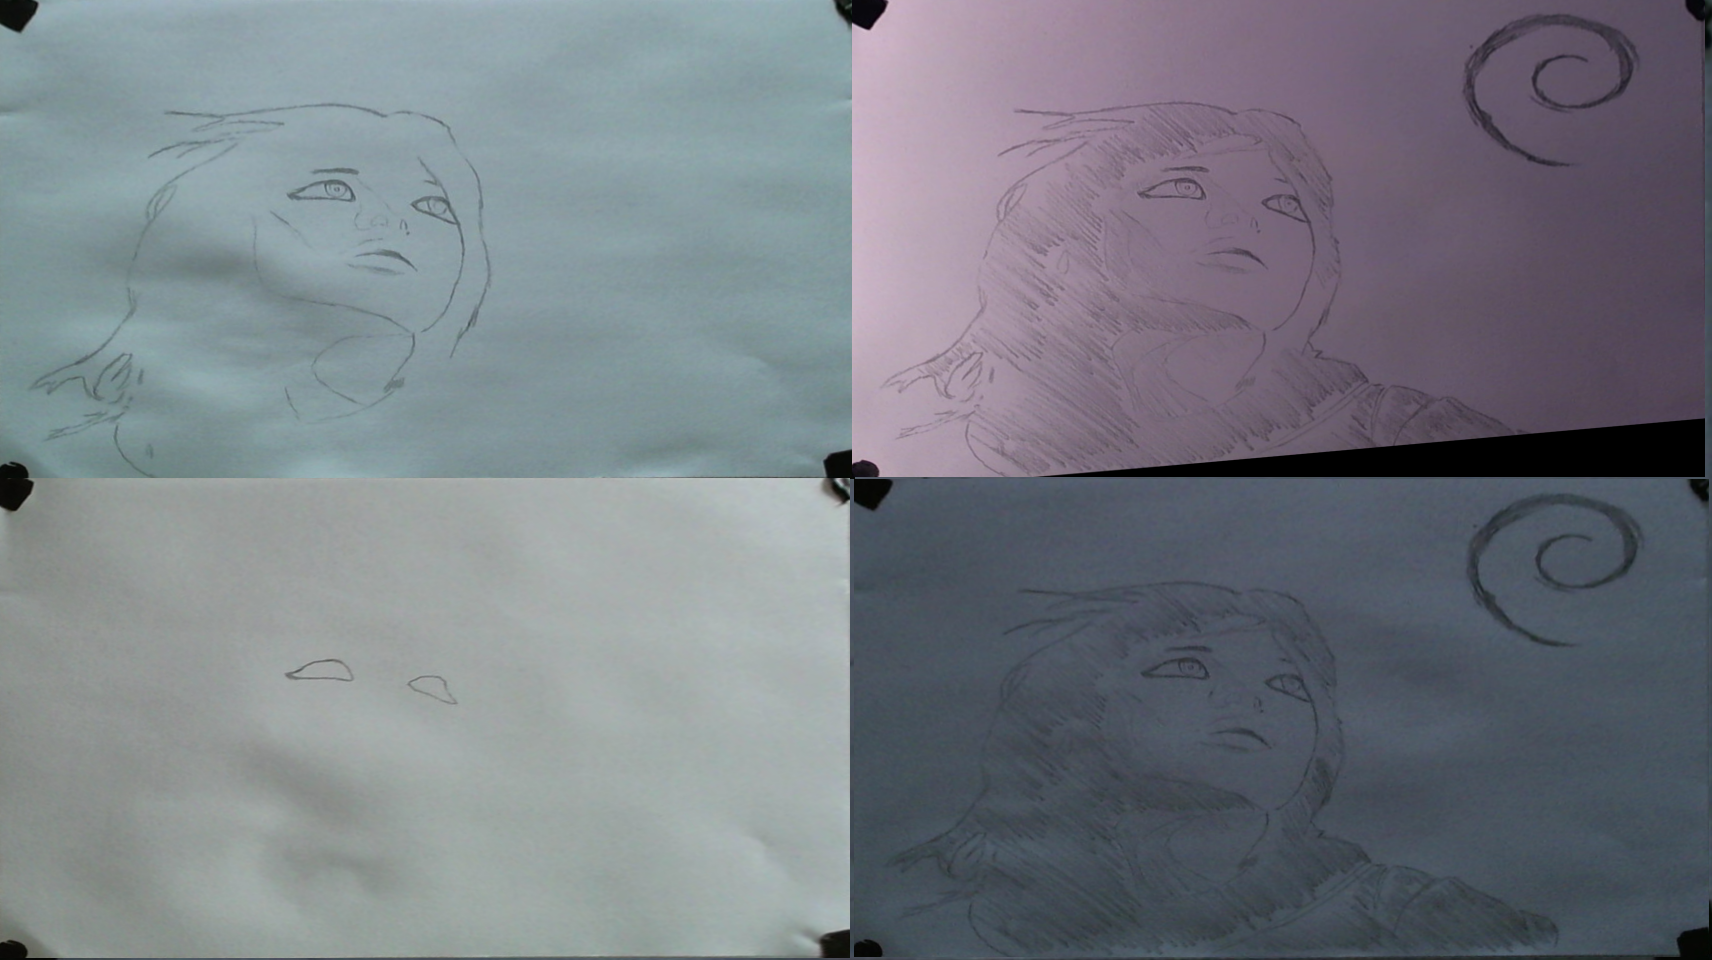
\includegraphics[scale=0.2]{images/diffEclairage.png}

%Un dessin est définit par un ensemble de trait et dans certain cas des zones %homogènes( coloriées) ce qui ne nous permet pas d'utiliser un filtre de détection de %contour. ce qui peut etre optimale pour un simple ensemble de trait  

\end{itemize}
\end{frame}

\vspace{5mm}
\begin{frame}{Méthodes utilisées}
\vspace{5mm}
\begin{itemize}[<+->]
\item Balance des blanc
\includegraphics<.>[scale=0.2]{images/wb.png}
%étirement d'histogramme sur chaques canals avant de les rassembler ==> 
%permet d'augmenter le contraste.
\item Seuillage local ( Méthode de Sauvola) 
\\Le seuil du pixel dépend de la moyenne et de l’écart type dans une fenêtre centré sur le pixel. 
\includegraphics<.>[scale=0.2]{images/sauvola.png}
%étude de l'article ... compare les méthodes de binarisation  
%formule 
%difficulté trait de faible intensité,  

\end{itemize}
\end{frame}

%\vspace{5mm}
%\begin{frame}{Sauvola}
%\vspace{5mm}
%
%\begin{equation}
%	S(i,j) = \mu(i,j) + \kappa.((\sigma(i,j)/R)-1))
%\end{equation}
%
%Avec :
%- S(i, j) : seuil à appliquer pour le point i, j ;\\
%- $\sigma(i, j)$ : valeur de l’écart type dans une fenêtre centré en i, j de taille $N * M$ ;\\
%- $\mu(i, j)$ : valeur moyenne des niveaux de gris dans la même fenêtre ;\\
%- $\kappa$ : constante fixée le plus généralement à 0, 2 ;\\
%- R : constante permettant d'ajuster la dynamique de l'ecart type, géneralement 128.
%- N et M appartenant à N.\\
%%article de ...
%%permet d'obtenir la moyenne en 2 additions et deux soustractions
%
%\end{frame}


\vspace{5mm}
\begin{frame}{Optimisation}
\vspace{5mm}
\begin{itemize}[<+->]
\item Image intégral
\\Reformulation par Viola et Jones "Robust real-time face detection" 2004
\includegraphics<.>[scale=0.25]{images/imageIntegrale1.png}
\item[]
\includegraphics<.>[scale=0.25]{images/imageIntegrale.png}
%article de ...
%permet d'obtenir la moyenne en 2 additions et deux soustractions
\end{itemize}
\end{frame}

%% part 3 - Nicolas
\section[Détection de Pictogrammes]{Détection de Pictogrammes}
\begin{frame}{Objectif}
\vspace{5mm}
\begin{itemize}
\item Développer un logiciel qui détecte des pictogrammes dans un flux vidéo.
\item Utilisation de templates représentant les pictogrammes.
\vspace{5mm}
\begin{center}
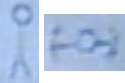
\includegraphics[scale=0.66]{images/templates.png}
\end{center}
\end{itemize}
\end{frame}

\begin{frame}{Méthode utilisée}
\vspace{5mm}
\begin{itemize}
\item Template Matching
\item Principe : 
\begin{center}
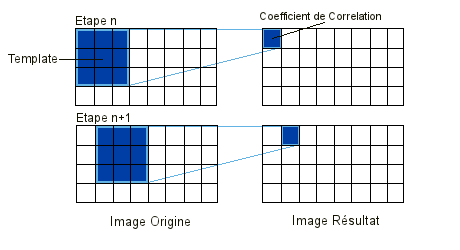
\includegraphics[scale=0.66]{images/templateMatching.png}
\end{center}
\end{itemize}
\end{frame}
			
\begin{frame}{Problème rencontré}
\vspace{5mm}
\begin{itemize}
\item \texttt{cvMatchTemplate} -> Carte de corrélation
\item Récupération du meilleur résultat
\item Difficulté pour déterminer un seuil d'acceptation
\end{itemize}
\end{frame}	

\begin{frame}{Résultats obtenus}
\vspace{5mm}
\begin{center}
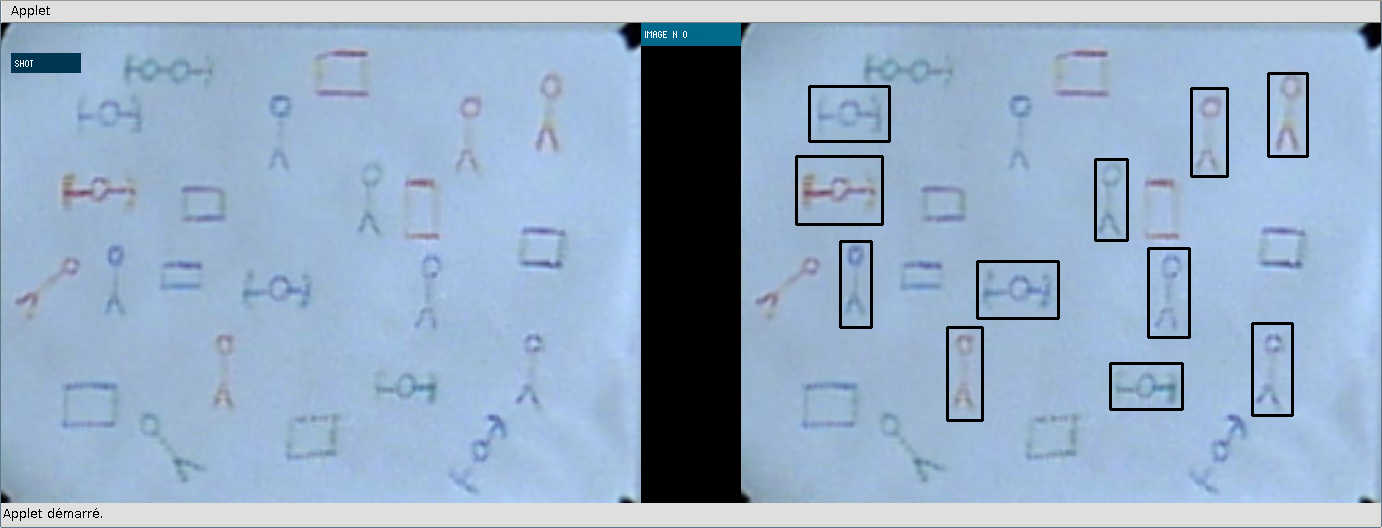
\includegraphics[width=\textwidth]{images/capture1.png}
\end{center}
\end{frame}

\begin{frame}{Résultats obtenus}
\vspace{5mm}
\begin{center}
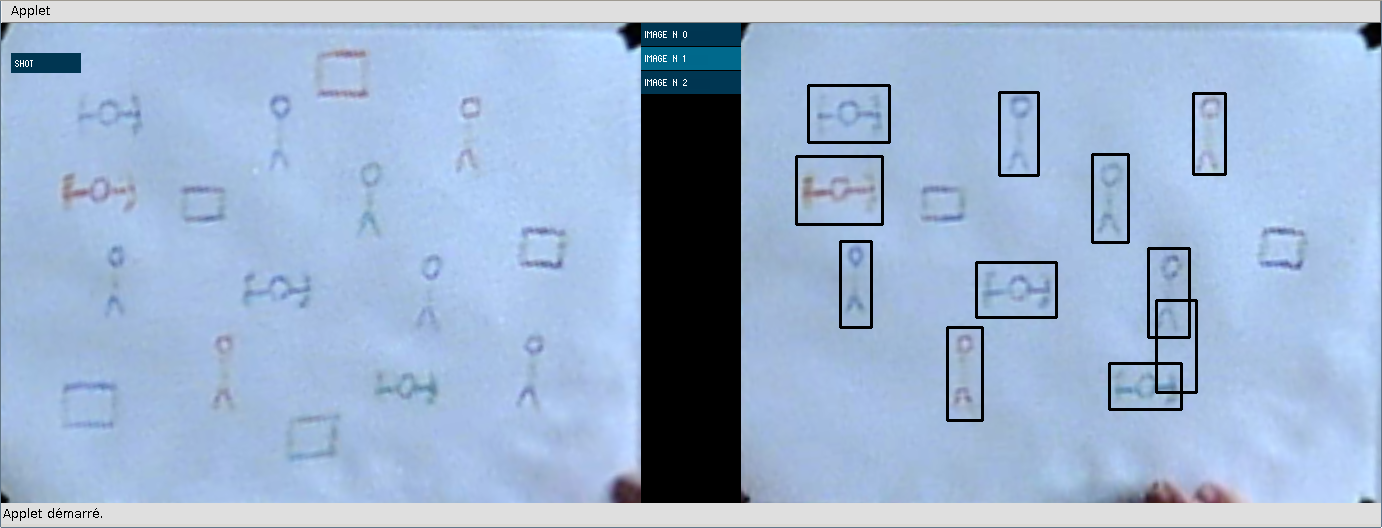
\includegraphics[width=\textwidth]{images/capture2.png}
\end{center}
\end{frame}

\begin{frame}{Méthode alternative}
\vspace{5mm}
\begin{itemize}
\item SURF
\item Intérêt : Non affecté par rotation et mise à l'échelle 
\item Problème : Qualité vidéo trop basse -> Trop peu de marqueurs détectés
\end{itemize}
\end{frame}
	
%% part 4 - Tomy
\section[Extraction de nouveautés]{Feature Extractor}
	\begin{frame}{Difficulties}
		\vspace*{5mm}
	\begin{itemize}
	\item Libraries installation
	\item Memory management
	\item Visualisation
	\end{itemize}
	\end{frame}
	
\section[Conclusion]{Conclusion}
	\begin{frame}{Conclusion}
		\vspace*{5mm}
		\begin{itemize}
		\item Software partially working
		\item A bad choice of buffer implementation
		\item Tests not done due to a lack of time
		\end{itemize}
	\end{frame}

\end{document}
